\documentclass[12pt,a4paper]{article}
\usepackage[utf8]{inputenc}
\usepackage[spanish]{babel}
\usepackage{geometry}
\usepackage{fancyhdr}
\usepackage{graphicx}
\usepackage{tabularx}
\usepackage{longtable}
\usepackage{booktabs}
\usepackage{amsmath}
\usepackage{amsfonts}
\usepackage{amssymb}
\usepackage{hyperref}
\usepackage{xcolor}
\usepackage{titlesec}

% Paquete para glosario
\usepackage[acronym,toc,nonumberlist]{glossaries}

% Configuración de página
\geometry{left=2.5cm,right=2.5cm,top=3cm,bottom=3cm}

% Configuración de encabezados y pies de página
\pagestyle{fancy}
\fancyhf{}
\fancyhead[L]{Propuesta Económica - UNICEF}
\fancyhead[R]{Empresa Kuya}
\fancyfoot[C]{\thepage}

% Configuración de títulos
\titleformat{\section}{\Large\bfseries\color{blue!70!black}}{\thesection}{1em}{}
\titleformat{\subsection}{\large\bfseries}{\thesubsection}{1em}{}

% Configuración de hipervínculos
\hypersetup{
    colorlinks=true,
    linkcolor=blue!70!black,
    filecolor=magenta,
    urlcolor=cyan,
    pdftitle={Propuesta Técnica UNICEF},
    pdfauthor={Empresa Kuya}
}

% Cargar definiciones del glosario
% =============================================================================
% GLOSARIO DE TÉRMINOS - PROPUESTA TÉCNICA UNICEF
% =============================================================================
% Este archivo contiene todas las definiciones de términos técnicos
% utilizados en la propuesta. Se utiliza el paquete glossaries para
% manejo automático de referencias y ordenamiento.
% =============================================================================

% Configuración del glosario
\makeglossaries

% =============================================================================
% TÉRMINOS TÉCNICOS GENERALES
% =============================================================================

\newglossaryentry{api}
{
    name={API},
    description={Application Programming Interface. Conjunto de protocolos, rutinas y herramientas para construir aplicaciones de software. Define las formas en que los componentes de software deben interactuar}
}

\newglossaryentry{backend}
{
    name={Backend},
    description={Parte del sistema que maneja la lógica del servidor, bases de datos y arquitectura de la aplicación. No es visible directamente para el usuario final}
}

\newglossaryentry{frontend}
{
    name={Frontend},
    description={Parte del sistema con la que interactúa directamente el usuario. Incluye la interfaz gráfica, navegación y experiencia del usuario}
}

\newglossaryentry{framework}
{
    name={Framework},
    description={Marco de trabajo o conjunto de herramientas, bibliotecas y convenciones que facilitan el desarrollo de aplicaciones de software}
}

\newglossaryentry{database}
{
    name={Base de Datos},
    description={Sistema organizado para almacenar, gestionar y recuperar información de manera eficiente y segura}
}

% =============================================================================
% METODOLOGÍAS Y PROCESOS
% =============================================================================

\newglossaryentry{agile}
{
    name={Metodología Ágil},
    description={Enfoque de desarrollo de software que enfatiza la colaboración, la flexibilidad y la entrega incremental de funcionalidades}
}

\newglossaryentry{scrum}
{
    name={Scrum},
    description={Marco de trabajo ágil para gestionar el desarrollo de productos complejos, basado en sprints y equipos autoorganizados}
}

\newglossaryentry{devops}
{
    name={DevOps},
    description={Conjunto de prácticas que combina desarrollo de software (Dev) y operaciones de TI (Ops) para acortar el ciclo de vida del desarrollo}
}

\newglossaryentry{cicd}
{
    name={CI/CD},
    description={Continuous Integration/Continuous Deployment. Práctica de automatizar la integración y despliegue de código para mejorar la calidad y velocidad de entrega}
}

% =============================================================================
% TECNOLOGÍAS WEB Y DESARROLLO
% =============================================================================

\newglossaryentry{html}
{
    name={HTML},
    description={HyperText Markup Language. Lenguaje de marcado estándar para crear páginas web y aplicaciones web}
}

\newglossaryentry{css}
{
    name={CSS},
    description={Cascading Style Sheets. Lenguaje utilizado para describir la presentación y el diseño de documentos HTML}
}

\newglossaryentry{javascript}
{
    name={JavaScript},
    description={Lenguaje de programación interpretado que permite crear contenido dinámico e interactivo en páginas web}
}

\newglossaryentry{nodejs}
{
    name={Node.js},
    description={Entorno de ejecución para JavaScript construido sobre el motor V8 de Chrome, que permite ejecutar JavaScript en el servidor}
}

\newglossaryentry{react}
{
    name={React},
    description={Biblioteca de JavaScript desarrollada por Facebook para construir interfaces de usuario, especialmente aplicaciones web de una sola página}
}

% =============================================================================
% BASES DE DATOS Y ALMACENAMIENTO
% =============================================================================

\newglossaryentry{sql}
{
    name={SQL},
    description={Structured Query Language. Lenguaje de programación diseñado para gestionar y manipular bases de datos relacionales}
}

\newglossaryentry{nosql}
{
    name={NoSQL},
    description={Término que describe bases de datos no relacionales diseñadas para manejar grandes volúmenes de datos y estructuras flexibles}
}

\newglossaryentry{mongodb}
{
    name={MongoDB},
    description={Sistema de base de datos NoSQL orientado a documentos, que almacena datos en formato similar a JSON}
}

\newglossaryentry{postgresql}
{
    name={PostgreSQL},
    description={Sistema de gestión de bases de datos relacionales y orientado a objetos de código abierto}
}

% =============================================================================
% SEGURIDAD Y AUTENTICACIÓN
% =============================================================================

\newglossaryentry{ssl}
{
    name={SSL/TLS},
    description={Secure Sockets Layer/Transport Layer Security. Protocolos criptográficos que proporcionan comunicaciones seguras por internet}
}

\newglossaryentry{oauth}
{
    name={OAuth},
    description={Estándar abierto para autorización que permite a aplicaciones de terceros obtener acceso limitado a servicios web}
}

\newglossaryentry{jwt}
{
    name={JWT},
    description={JSON Web Token. Estándar para transmitir información de forma segura entre partes como un objeto JSON compacto y autónomo}
}

\newglossaryentry{https}
{
    name={HTTPS},
    description={HyperText Transfer Protocol Secure. Protocolo de comunicación seguro que utiliza cifrado SSL/TLS para proteger la transferencia de datos}
}

% =============================================================================
% ARQUITECTURA Y INFRAESTRUCTURA
% =============================================================================

\newglossaryentry{microservices}
{
    name={Microservicios},
    description={Arquitectura de software que estructura una aplicación como un conjunto de servicios pequeños, independientes y débilmente acoplados}
}

\newglossaryentry{docker}
{
    name={Docker},
    description={Plataforma de virtualización a nivel de sistema operativo que permite empaquetar aplicaciones y sus dependencias en contenedores}
}

\newglossaryentry{kubernetes}
{
    name={Kubernetes},
    description={Sistema de orquestación de contenedores de código abierto para automatizar el despliegue, escalado y gestión de aplicaciones}
}

\newglossaryentry{cloud}
{
    name={Cloud Computing},
    description={Entrega de servicios de computación a través de internet, incluyendo servidores, almacenamiento, bases de datos y software}
}

\newglossaryentry{aws}
{
    name={AWS},
    description={Amazon Web Services. Plataforma de servicios en la nube que ofrece potencia de cómputo, almacenamiento de bases de datos y distribución de contenido}
}

% =============================================================================
% TÉRMINOS ESPECÍFICOS DE UNICEF
% =============================================================================

\newglossaryentry{beneficiario}
{
    name={Beneficiario},
    description={Persona que recibe directamente los servicios, programas o asistencia proporcionados por UNICEF}
}

\newglossaryentry{programa}
{
    name={Programa},
    description={Conjunto coordinado de actividades diseñadas para lograr objetivos específicos de desarrollo infantil y protección de derechos}
}

\newglossaryentry{monitoreo}
{
    name={Monitoreo},
    description={Proceso sistemático de recolección y análisis de información para seguir el progreso de programas y actividades}
}

\newglossaryentry{indicador}
{
    name={Indicador},
    description={Medida cuantitativa o cualitativa que proporciona información sobre el progreso hacia el logro de objetivos específicos}
}

% =============================================================================
% GESTIÓN DE PROYECTOS
% =============================================================================

\newglossaryentry{sprint}
{
    name={Sprint},
    description={Período de tiempo fijo (generalmente 1-4 semanas) durante el cual se completa un conjunto específico de trabajo en metodologías ágiles}
}

\newglossaryentry{stakeholder}
{
    name={Stakeholder},
    description={Persona, grupo u organización que puede afectar o ser afectado por las actividades y decisiones de un proyecto}
}

\newglossaryentry{milestone}
{
    name={Hito (Milestone)},
    description={Punto significativo en el cronograma del proyecto que marca la finalización de una fase o entregable importante}
}

\newglossaryentry{deliverable}
{
    name={Entregable},
    description={Producto, servicio o resultado único y verificable que debe ser producido para completar un proceso, fase o proyecto}
}

% =============================================================================
% CALIDAD Y TESTING
% =============================================================================

\newglossaryentry{qa}
{
    name={QA},
    description={Quality Assurance. Proceso sistemático para determinar si un producto o servicio cumple con los requisitos especificados}
}

\newglossaryentry{unittest}
{
    name={Prueba Unitaria},
    description={Método de testing que verifica el funcionamiento correcto de componentes individuales del software}
}

\newglossaryentry{uat}
{
    name={UAT},
    description={User Acceptance Testing. Fase final de testing donde usuarios finales verifican que el sistema cumple con sus requisitos}
}

\newglossaryentry{regression}
{
    name={Prueba de Regresión},
    description={Tipo de testing que verifica que nuevos cambios no afecten negativamente funcionalidades existentes}
}

% =============================================================================
% INTERFAZ Y EXPERIENCIA DE USUARIO
% =============================================================================

\newglossaryentry{ui}
{
    name={UI},
    description={User Interface. Interfaz de usuario que abarca todos los elementos visuales e interactivos con los que el usuario interactúa}
}

\newglossaryentry{ux}
{
    name={UX},
    description={User Experience. Experiencia global que tiene una persona al usar un producto, sistema o servicio}
}

\newglossaryentry{responsive}
{
    name={Diseño Responsivo},
    description={Enfoque de diseño web que hace que las páginas se vean bien en todos los dispositivos y tamaños de pantalla}
}

\newglossaryentry{wireframe}
{
    name={Wireframe},
    description={Representación esquemática de la estructura y funcionalidad de una página web o aplicación, sin elementos de diseño visual}
}

% =============================================================================
% COMANDO PARA IMPRIMIR EL GLOSARIO
% =============================================================================
% Para incluir el glosario en el documento principal, usar:
% \printglossary[title={Glosario de Términos}]

\begin{document}

% Incluir portada
\begin{titlepage}
    \centering
    
    \vspace{2cm}
    
    % Título principal
    {\Huge\bfseries PROPUESTA ECONÓMICA\\[0.5cm]}
    {\Large\bfseries Desarrollo de Solución Tecnológica\\[0.3cm]}
    {\Large para UNICEF\\[2cm]}
    
    % Subtítulo
    {\large\textit{Cotización y Estructura de Costos\\
    para Sistema Digital Integral}\\[3cm]}
    
    % Información de la empresa
    {\Large\bfseries EMPRESA KUYA\\[0.5cm]}
    {\large Soluciones Tecnológicas Innovadoras\\[2cm]}
    
    % Fecha
    {\large\textbf{Fecha:} 25 de Octubre de 2025\\[1cm]}
    
    % Información adicional
    {\normalsize
    \textbf{Dirigido a:} Fondo de las Naciones Unidas para la Infancia (UNICEF)\\[0.3cm]
    \textbf{Versión:} 1.0\\[0.3cm]
    \textbf{Tipo:} Propuesta Económica\\
    }
    
    \vfill
    
    % Pie de página
    {\footnotesize
    Este documento contiene información comercial confidencial.\\
    Su distribución está restringida únicamente a personal autorizado de UNICEF.
    }
    
\end{titlepage}

\newpage
\thispagestyle{empty}
\mbox{}
\newpage

% Tabla de contenidos
\tableofcontents
\newpage

% Incluir secciones
\newpage

\section{Objetivos}

\subsection{Objetivo Principal}
Desarrollar e implementar la mejora y reestructuración del Sistema de Alerta Temprana (SAT) del Ministerio de Educación, Deporte y Cultura, mediante una plataforma web tecnológica modular, escalable y de acceso web, que permita gestionar, analizar y visualizar información sobre eventos adversos que afectan al sistema educativo, facilitando la toma de decisiones oportunas, conforme a los lineamientos técnicos establecidos.

\subsection{Objetivos Específicos}

\begin{enumerate}
    \item \textbf{Reestructuración y mejora de la plataforma:} Corregir errores, reestructurar y mejorar integralmente la Plataforma del SAT sobre su base tecnológica actual, asegurando su funcionamiento en una plataforma web accesible por internet.
    
    \item \textbf{Arquitectura escalable:} Implementar una arquitectura modular escalable que soporte la futura incorporación de aproximadamente 4 módulos adicionales y un aplicativo móvil.
    
    \item \textbf{Funcionalidades de gestión:} Integrar funcionalidades robustas como registro, gestión, y análisis de información relacionada con eventos adversos.
    
    \item \textbf{Integración de sistemas:} Integrar datos georreferenciados, automatizar reportes y garantizar la interoperabilidad con sistemas institucionales como AMIE y GIEE.
    
    \item \textbf{Implementación de módulos funcionales:} Implementar tres módulos funcionales en la primera fase: ADMINISTRACIÓN, EVENTOS ADVERSOS y VISUALIZADOR.
    
    \item \textbf{Sistema de roles:} Desarrollar la plataforma con roles diferenciados (Técnico de Riesgos Distrital, Zonal y Nacional) para una gestión descentralizada y eficiente.
    
    \item \textbf{Trazabilidad de información:} Garantizar la trazabilidad de la información de eventos, incluyendo la edición, revisión, y aprobación según el rol del usuario.
    
    \item \textbf{Capacitación:} Diseñar e implementar un plan de capacitación técnica y funcional a funcionarios y usuarios del SAT.
\end{enumerate}

\newpage

El alcance principal es la mejora funcional y reestructuración del SAT a través del desarrollo e implementación de nuevos módulos y la reestructuración de los existentes. El desarrollo debe realizarse sobre la base tecnológica actual del SAT, garantizando interoperabilidad con sistemas institucionales, trazabilidad y escalabilidad
\newpage

\section{Perfil de la Institución}
\label{sec:perfil_institucion}

\subsection{Información General}

KUYACODE S.A.S, es una empresa Ecuatoriana generadora de soluciones tecnológicas innovadoras, fundada en 2025, conformada por un equipo multidisciplinario con más de 10 años de experiencia en el desarrollo de software y consultoría tecnológica. Nuestra misión es proporcionar soluciones que impulsen la eficiencia y la innovación en diversas industrias, incluyendo el sector humanitario.

\subsection{Experiencia Relevante}

Como consultores independientes a lo largo de nuestra trayectoria, hemos trabajado con múltiples organizaciones internacionales, incluyendo agencias de la ONU, ONGs y entidades gubernamentales. como empresa KUYACODE S.A.S, hemos participado en 2 proyecto elevantes.

Algunos de nuestros proyectos más destacados incluyen:
\begin{itemize}
    \item \textbf{2021 Implementación de la plataforma DHIS2}\footnote{ District Health Information System, Sistema de información de salud distrital}
    
        En el 2021 y parte del 2022 bajo el auspicio de la OPS/OMS, participamos en la implementación de la plataforma DHIS2 (District Health Information System) para el Ministerio de Salud Pública de Ecuador, con el objetivo de mejorar la gestión y análisis de datos de salud a nivel nacional.

        La plataforma DHIS2 fue implementada para recopilar los datos nominales de vacunación COVID-19 y ESAVIS en todo el país a nivel de establecimiento, permitiendo un seguimiento más eficiente de las campañas de vacunación y la gestión de eventos adversos relacionados con la inmunización.

        La configuración de la plataforma incluyó la integración con los servicios del Registro Civil, para la agilización y registro automático de datos de los pacientes vacunados, cono nombres, apellidos, cédula de identidad, fecha de nacimiento, sexo, estado civil.

        Incluyo tambien la integración con la plataforma de distribución de establecimientos de salud del Ministerio de Salud Pública, para la gestión y actualización automática de la información de los establecimientos de salud a nivel nacional.

        Nuestra labor incluyó la configuración del sistema, capacitación del personal y soporte técnico continuo para asegurar una adopción efectiva de la plataforma.

    \item \textbf{2022, Sistema de información Regional ESAVIS}\footnote{Evento Supuestamente Atribuible a la Vacunación o Inmunización} 

        Con el auspicio de la OPS/OMS REGIONAL, brindamos consultorías especializadas para la implementación de sistemas de información de ESAVIS REGIONAL en Paraguay, Ecuador y El Salvador.

        Las consulorias incluyeron el análisis de requerimientos, diseño e implementación de la plataforma tecnológicas para el registro de los eventos supuestamente atribuibles a la vacunación o inmunización (ESAVIS) ajustados a la realidad tecnológica de cada país.

        Las implementaciones brindaron un mecanismo para la notificación regional de ESAVIS, permitiendo el analisis y monitoreo de los eventos relacionados con la vacunación de una forma estandarizada y eficiente.
        
        Los sistemas implementados permiten la integración y estandarización de datos, de las deferentes fuentes, mejorando la eficiencia y efectividad de los programas de vacunación en los países beneficiarios.
    
    \item \textbf{2024 - Actualidad, YAKU, IUSTITIA PERMANENS}.

        KUYACODE S.A.S ha brindado servicios de consultoría al consorcio de abogados IUSTITIA PERMANENS, Abg Asociados para el desarrollo de la plataforma multitenant de registro y monitoreo de consumo de agua potable comunitaria YAKU. El proyecto YAKU constituye una solución tecnológica integral que permite el registro, monitoreo y análisis del consumo de agua potable en comunidades rurales, facilitando la toma de decisiones informadas para mejorar la gestión del recurso hídrico.

        El sistema incluye una aplicación móvil para la recolección de datos en campo en modo desconectado, es utilizando para el registro de de las lecturas de consumo de agua en los medidores. 

        La plataforma gestiona el registro de clientes, acometidas, medidores, predios, consumos de agua, generación de facturas y reportes contables, proporcionando una herramienta completa para la administración de servicios de agua potable en entornos comunitarios.

        La plataforma incluye una aplicación movil para la recolección de datos en campo en modo desconectado, es utilizando para el registro de de las lecturas de consumo de agua en los medidores por parte de los operadores, facilitando la labor de recolección de datos en entornos rurales.

        Actualmente, la plataforma YAKU se encuentra implementada para la comunidad de AINCHE, ubicada en la provincia de Chimborazo, Ecuador, y está en proceso de expansión a otras comunidades.

        URL: \url{https://yaku.kuyacode.com}

    \item \textbf{2024-2025, Plataforma de Monitoreo de Flota y Logística}

        KUYACODE S.A.S ha brindado servicios de consultoría a la empresa QUALITYFAST S.A. en el desarrollo y mejora de su plataforma de monitoreo en tiempo real de vehículos y logística en transporte. Esta plataforma permite a QUALITYFAST S.A. rastrear y gestionar eficientemente su flota de vehículos, optimizando las operaciones logísticas y mejorando la eficiencia del transporte.

        La plataforma incluye funcionalidades avanzadas de seguimiento GPS, gestión de rutas, monitoreo en tiempo real de vehículos, gestión de alertas y notificaciones, gestiones de flotas, contratos, clientes, responsables, dispositivos, entre otros.
        
        Actualmente QUALITYFAST S.A está migrando su anterior plataforma a esta nueva versión que implementa una nueva arquitectura basada en microservicios para mejorar su escalabilidad y rendimiento, ademas de integrar nuevas funcionalidades, mejoras funcionales y de seguridad.

        URL: \url{http://rastreoweb.net/}, \url{http://devtenant1.rastreoweb.com/}
\end{itemize}

\subsection{Referencias}
Podemos proporcionar referencias de nuestros clientes.
\begin{itemize}
    \item \textbf{IUSTITIA PERMANENS, Abg Asociados:} Proyecto YAKU
    \begin{itemize}
        \item Abg. Ricardo Parra Chavez
        \item Teléfono: +593 98 764 9183
        \item Correo Electrónico: ricardo.parra@gad.com
    \end{itemize}
    \item \textbf{Ing. Francisco Quiroga, CEO} Proyecto QUALITYFAST S.A., Rastreo Vehicular y Logística
    \begin{itemize}
        \item Ing. Francisco Quiroga
        \item Teléfono: +593 99 929 3029
        \item Correo Electrónico: fastq2000@gmail.com
    \end{itemize}
\end{itemize}
\subsection{Perfiles del Equipo}
Nuestro equipo está compuesto por profesionales con experiencia en el desarrollo de software, gestión de proyectos, análisis de datos y consultoría tecnológica. A continuación, se listan los perfiles considerados para el participación en este proyecto:
\begin{itemize}
        \item \textbf{Ing. Rolando Vinicio Casigña Parra} - CEO, Arquitecto de Soluciones: Con 13 años de experiencia en desarrollo de software y gestión de proyectos tecnológicos. Actualmente involucrado en soluciones de análisis de datos y trabajo de datos. con experiencia en tecnologías JAVA, nodejs, python, bases de datos relacionales.\\
        \textbf{Participación:} Presencial, Lidera la estrategia técnica y supervisa la implementación de soluciones, asegurando el cumplimiento de los objetivos del proyecto.
        \item \textbf{Msg. Eco. Nataly Paulina Verdugo Morales} - PM: Economista con 15 años de experiencia en la gestión de proyectos de análisis económico, trabajo con recursos humanos y gestión logistica.\\
        \textbf{Participación:} Presencial, Responsable de la gestión del proyecto, coordinación con UNICEF y supervisión del cumplimiento de los objetivos.\\
        \item \textbf{Msg. Ing. Nelson López Naranjo} - Lider Técnico: Ingeniero en sistemas con más de 15 años de experiencia en desarrollo de software y gestión de equipos técnicos, especialista de arquitecturas de software y metodologias ágiles, con experiencia y manejo de tecnologías JAVA, nodejs, bases de datos relacionales. \\
        \textbf{Participación:} Remoto, Lidera el equipo técnico y supervisa la implementación de soluciones. \\
        \item \textbf{Msg. Ing. Roberto Maldonado Palacios} - Desarrollador Full Stack: Ingeniero en sistemas con 15 años de experiencia en desarrollo de software, especializado en aplicaciones web y móviles, experiencia con tecnologías front-end y back-end con lenguajes JAVA, nodejs, angular, react. \\
        \textbf{Participación:} Remoto, Desarrolla e implementa la solución web según los requerimientos del proyecto.\\
        \item \textbf{Msg. Ing. Ximena Celi Celi} - Analista de datos: Ingeniera en sistemas con experiencia en análisis de datos y visualización, especializada en herramientas opensource Python, streamlit, jasperReports.\\
        \textbf{Participación:} Remoto, Desarrolla e implementa la solución  de analítica según los requerimientos del proyecto.\\
        \item  \textbf{Ing. Ivette Carolina Castrillon Zamora} - Especialista en Aseguramiento de Calidad: Ingeniera en sistemas con experiencia en pruebas de software, automatización de pruebas y aseguramiento de calidad, con conocimientos en herramientas como Selenium, JUnit, k6.\\
        \textbf{Participación:} Remoto, Responsable de diseñar y ejecutar las pruebas funcionales y no funcionales del sistema.
\end{itemize}
Las hojas de vida detalladas de cada miembro del equipo están disponibles en los anexos de este documento.
\newpage

\section{Metodología de Desarrollo}

\subsection{Enfoque Metodológico}

Para el desarrollo de este proyecto se adoptará una metodología ágil basada en \textbf{Scrum}, que permitirá una entrega iterativa e incremental de los productos, garantizando la adaptabilidad a los cambios y la participación activa del cliente durante todo el proceso de desarrollo.

\subsection{Fases del Proyecto}

Tomando en cuenta las fases planteadas en los terminos de referencia, se ajustará la metodología para cumplir con los entregables y cronogramas establecidos.\\
A continuación, se describen las fases del proyecto junto con los principales actores involucrados en cada una de ellas:

\begin{itemize}
    \item \textbf{Producto 1}: Documento de diagnóstico, restructuración y mejora del sistema de alerta temprana SAT (Plan de trabajo).

    Principales actores:
    \begin{table}[h]
        \centering
        \begin{tabular}{|p{3cm}|p{5cm}|p{7cm}|}
            \hline
            \textbf{Rol} & \textbf{Entidad} & \textbf{Descripción} \\
            \hline
            Coordinador Técnico & Ministerio de Educación & Enlace técnico y validador de los entregables por parte del cliente \\
            \hline
            Arquitecto de Software & KUYACODE & Encargado del diseño de la arquitectura técnica y tecnológica del sistema \\
            \hline
            Administrador de Proyectos (PM) & KUYACODE & Responsable de la gestión, planificación y seguimiento del proyecto \\
            \hline
        \end{tabular}
        \caption{Principales actores involucrados en el Producto 1}
        \label{tab:actores_producto1}
    \end{table}
    
    \item \textbf{Producto 2}: Documento para el rediseño del Sistema de Alerta Temprana SAT conforme a los lineamientos del Ministerio de Educación, Deporte y Cultura.\\
    \begin{table}[htbp]
        \centering
        \begin{tabular}{|p{3cm}|p{5cm}|p{7cm}|}
            \hline
            \textbf{Rol} & \textbf{Entidad} & \textbf{Descripción} \\
            \hline
            Coordinador Técnico & Ministerio de Educación & Enlace técnico y validador de los entregables por parte del cliente \\
            \hline
            Arquitecto de Software & KUYACODE & Responsable de recopilar y documentar los requerimientos funcionales y no funcionales del sistema \\
            \hline
            Administrador de proyecto& KUYACODE & Responsable de la gestión y comunicación del proyecto e involucrados \\
            \hline
        \end{tabular}
        \caption{Principales actores involucrados en el Producto 2}
        \label{tab:actores_producto2}
    \end{table}
    \\

    \item \textbf{Producto 3}: Correcciones, reestructuración y mejora de la plataforma de acuerdo con el detalle de Requerimiento Funcional sobre la plataforma de Desarrollo proporcionada por el Ministerio de Educación, Deporte y Cultura.\\

    \begin{table}[h]
        \centering
        \begin{tabular}{|p{3cm}|p{5cm}|p{7cm}|}
            \hline
            \textbf{Rol} & \textbf{Entidad} & \textbf{Descripción} \\
            \hline
            Coordinador Técnico & Ministerio de Educación & Enlace técnico y validador de los entregables por parte del cliente \\
            \hline
            Administrador de proyecto & KUYACODE & Responsable de la gestión y comunicación del proyecto e involucrados \\
            \hline
            Arquitecto de Software & KUYACODE & Responsable de la definición de la arquitectura técnica y tecnológica del sistema, desarrollo de prototipos y validación de soluciones \\
            \hline
            Desarrollador Senior & KUYACODE & Encargado de la implementación de las correcciones y mejoras funcionales definidas en los terminos de referencia y levantamiento de requerimientos \\
            \hline
            Desarrollador Senior WEB & KUYACODE & Encargado de la implementación de las correcciones y mejoras funcionales web definidas en los terminos de referencia y levantamiento de requerimientos \\
            \hline
            Analista de datos & KUYACODE & Encargado de la implementación de la analítica de datos del sistema \\
            \hline
        \end{tabular}
        \caption{Principales actores involucrados en el Producto 3}
        \label{tab:actores_producto3}
        \end{table}

    \item \textbf{Producto 4}: Informe de pruebas del funcionamiento del Sistema de Alerta Temprana SAT.\\
    
    \begin{table}[htbp]
        \centering
        \begin{tabular}{|p{3cm}|p{5cm}|p{7cm}|}
            \hline
            \textbf{Rol} & \textbf{Entidad} & \textbf{Descripción} \\
            \hline
            Coordinador Técnico & Ministerio de Educación & Validador de los resultados de pruebas por parte del cliente \\
            \hline
            Administrador de proyecto & KUYACODE & Responsable de la gestión y comunicación del proyecto e involucrados \\
            \hline
            QA Engineer & KUYACODE & Responsable de diseñar y ejecutar las pruebas funcionales y no funcionales del sistema \\
            \hline
            Arquitecto de Software & KUYACODE & Supervisor técnico de las pruebas y validación de resultados \\
            \hline
        \end{tabular}
        \caption{Principales actores involucrados en el Producto 4}
        \label{tab:actores_producto4}
    \end{table}

    \item \textbf{Producto 5}: Informe de implementación definitiva del sistema en un ambiente productivo.\\
    
    \begin{table}[h]            
        \centering
        \begin{tabular}{|p{3cm}|p{5cm}|p{7cm}|}
            \hline
            \textbf{Rol} & \textbf{Entidad} & \textbf{Descripción} \\
            \hline
            Administrador de Sistemas & Ministerio de Educación & Responsable de la infraestructura y soporte del ambiente productivo \\
            \hline
            Coordinador Técnico & KUYACODE & Responsable del despliegue y configuración en ambiente productivo \\
            \hline
            Administrador de Proyectos (PM) & KUYACODE & Coordinador de la implementación y seguimiento de actividades \\
            \hline
        \end{tabular}   
        \caption{Principales actores involucrados en el Producto 5}
        \label{tab:actores_producto5}
    \end{table}

    \item \textbf{Producto 6}: Plan de capacitación que incluya fechas de las sesiones de capacitación acordadas, aprobado por la Dirección de Gestión de Riesgos.
    
    \begin{table}[h]
        \centering
        \begin{tabular}{|p{3cm}|p{5cm}|p{7cm}|}
            \hline
            \textbf{Rol} & \textbf{Entidad} & \textbf{Descripción} \\
            \hline
            Capacitador Técnico & KUYACODE & Responsable del diseño e impartición de las capacitaciones técnicas \\
            \hline
            Administrador de Proyectos (PM) & KUYACODE & Impartir las capacitaciones funcionales y supervisar su ejecución \\
            \hline
            Arquitecto de software & KUYACODE & Impartir las capacitaciones técnicas y supervisar su ejecución \\
            \hline
        \end{tabular}
        \caption{Principales actores involucrados en el Producto 6}
        \label{tab:actores_producto6}
    \end{table} 
    \item \textbf{Producto 7}: Informe de soporte técnico que incluya los ajustes realizados. Acta de cierre técnico aprobada por la Dirección de Gestión de Riesgos y la Coordinación Nacional de TICS.

    \begin{table}[h]
        \centering
        \begin{tabular}{|p{3cm}|p{5cm}|p{7cm}|}
            \hline
            \textbf{Rol} & \textbf{Entidad} & \textbf{Descripción} \\
            \hline
            Soporte Técnico & KUYACODE & Responsable de brindar soporte técnico y realizar ajustes necesarios \\
            \hline
            Administrador de Proyectos (PM) & KUYACODE & Coordinador del cierre técnico y documentación final \\
            \hline
            Director de Gestión de Riesgos & Ministerio de Educación & Aprobador del acta de cierre técnico \\
            \hline
            Coordinador Nacional de TICS & Ministerio de Educación & Co-aprobador del acta de cierre técnico \\
            \hline
        \end{tabular}
        \caption{Principales actores involucrados en el Producto 7}
        \label{tab:actores_producto7}
    \end{table}
    \item \textbf{Producto 8}: Certificado de garantía de funcionamiento.
    \begin{table}[ht]
        \centering
        \begin{tabular}{|p{3cm}|p{5cm}|p{7cm}|}
            \hline
            \textbf{Rol} & \textbf{Entidad} & \textbf{Descripción} \\
            \hline
            Gerente de Proyecto & KUYACODE & Responsable de emitir el certificado de garantía y comprometerse con el soporte \\
            \hline
            Arquitecto de Software & KUYACODE & Validador técnico de la calidad y funcionamiento del sistema \\
            \hline
            Director de Gestión de Riesgos & Ministerio de Educación & Receptor y validador del certificado de garantía \\
            \hline
        \end{tabular}
        \caption{Principales actores involucrados en el Producto 8}
        \label{tab:actores_producto8}
    \end{table}
\end{itemize}
\subsection{Herramientas y Tecnologías}
\subsubsection{Gestión de Proyecto}
La propuesta incluye la intervención de un Administrador de proyectos (PM) que utilizará herramientas ágiles para la gestión y seguimiento del proyecto, tales como:
\begin{itemize}
    \item \textbf{Libre Project}: Gestión de proyectos, para la planificación y seguimiento de tareas, hitos y recursos del proyecto.
    \item \textbf{Confluence}: Plataforma de colaboración para la documentación del proyecto, permitiendo la creación y gestión de documentos técnicos, actas de reuniones y otros recursos relevantes.
    \item \textbf{skalydraw}: Herramienta para la creación de diagramas y flujogramas que faciliten la visualización de procesos y arquitecturas del sistema.
\end{itemize}
\subsubsection{Control de Versiones}
El manejo del código fuente se realizará utilizando las siguientes herramientas:
\begin{itemize}
    \item \textbf{Git}: Plataforma de control de versiones gestionado por el ministerio Ministerio de Educación, Cultura y deporte, con acceso para los desarrolladores y el equipo de QA.
    Si el Ministerio de Educación lo requiere, se creará una organización en GitHub con acceso privado a un equipo limitado.
\end{itemize}
\subsubsection{Documentación}
La documentación generada del proyecto será almacenada y gestionada utilizando:
\begin{itemize}
    \item \textbf{Git-Wiki}: Permite generar una wiki con la documentación del proyecto, asi tambien el versionamiento del mismo.
    \item \textbf{Swagger}: Documentación de APIs RESTful, permitiendo una fácil comprensión y uso por parte de los desarrolladores y clientes de las aplicaciones.
    \item \textbf{Docs}: Generador de documentación técnica a partir de comentarios en el código fuente.
\end{itemize}
\subsubsection{Desarrollo y Testing}
El desarrollo y testing se realizará utilizando las siguientes herramientas y tecnologías:
\begin{itemize}
    \item \textbf{IDE}: Visual Studio Code, IntelliJ IDEA, Eclipse IDEA
    \item \textbf{Lenguajes de Programación}: Java, JavaScript/TypeScript, Python
    \item \textbf{Frameworks}: Spring Boot, React, Angular, Node.js
    \item \textbf{Testing}: Jest, JUnit, Selenium
\end{itemize}
\subsection{Aseguramiento de Calidad}
La validación y aseguramiento de la calidad del software se llevará a cabo mediante las siguientes prácticas:
\begin{itemize}
    \item \textbf{Codestyler}: Herramienta para el análisis y formateo del código fuente, asegurando el cumplimiento de las convenciones de estilo.
    \item \textbf{SonarQube}: Análisis estático de código para identificar vulnerabilidades, bugs y code smells.
    \item \textbf{Pruebas Unitarias}: Implementación de pruebas unitarias para validar el correcto funcionamiento de los componentes individuales del software integradas en la construcción de la solución.
    \item \textbf{Pruebas de integración}: Validación de la interacción entre diferentes módulos del sistema.
    \item \textbf{Pruebas de aceptación}: Validación final por parte del cliente para asegurar que el producto cumple con los requerimientos especificados mediante la revisión y aprobación funcional.
\end{itemize}
\subsubsection{Proceso de Testing}
La estrategia de testing incluirá:
\begin{itemize}
    \item \textbf{Pruebas automatizadas}: Unitarias, integración y funcionales
    \item \textbf{Pruebas manuales}: Exploratorias y de usabilidad
    \item \textbf{Performance testing}: Pruebas de carga y rendimiento
\end{itemize}
\subsection{Comunicación y Seguimiento}
La comunicación efectiva y el seguimiento del proyecto se considera una parte fundamental para el éxito del mismo. El acompañamiento de un Administrador de proyectos (PM) garantizará una comunicación fluida entre el equipo de desarrollo y el cliente, así como un seguimiento riguroso del progreso del proyecto.\\
La participación activa del equipo de KUYACODE y del Ministerio de Educación en las reuniones de seguimiento permitirá una rápida identificación y resolución de problemas, asegurando que el proyecto se mantenga en línea con los objetivos y plazos establecidos.\\
Identificar puntos focales con asignación de responsabilidades permitirá garantizar la comunicación y toma de decisiones efectivas.
\subsubsection{Reuniones Regulares}
Para la gestión efectiva del proyecto, la propuesta incluye la realización de reuniones regulares para el seguimiento del proyecto, incluyendo:
\begin{itemize}
    \item \textbf{Daily Standup}: Reuniones diarias de 15 minutos, con el equipo de desarrollo para revisar el progreso y obstáculos, con la participación del PM, desarrolladores y líderes técnicos y contraparte funcional.
    \item \textbf{Sprint Planning}: Planificación al inicio de cada sprint, reunión para definir las tareas y objetivos del sprint cada 15 días. con los participación de el PM, desarrolladores, líderes técnicos y contraparte funcional.
    \item \textbf{Sprint Review}: Demostración al final de cada sprint cada 5 días.
\end{itemize}
\subsubsection{Reportes y Métricas}
Mediante el uso de herramientas de gestión de proyectos OpenProject se podra brindar un seguimiento detallado del avance y actividades del proyecto a través de de su herramienta web:
\subsection{Gestión de Riesgos}
\begin{itemize}
    \item Identificación temprana de riesgos técnicos y de proyecto
    \item Plan de contingencia para escenarios críticos
    \item Backup y recuperación de datos
    \item Documentación de decisiones técnicas importantes
\end{itemize}
\newpage

\section{Arquitectura de la Solución}

\subsection{Visión General de la Arquitectura}

La arquitectura propuesta para el sistema KUYA-UNICEF se basa en un enfoque modular y escalable que garantiza la flexibilidad, mantenibilidad y rendimiento del sistema. La solución adopta una arquitectura de microservicios con patrones modernos de desarrollo.

\begin{figure}[h]
\centering
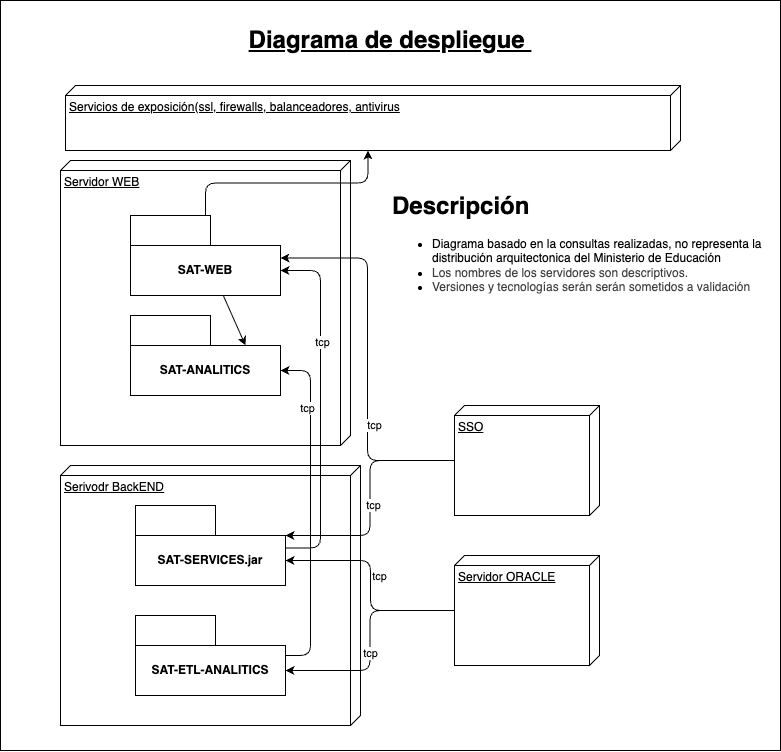
\includegraphics[width=0.8\textwidth]{graficos/arquitectura.png}
\caption{Propuesta de Diagrama de Arquitectura de la Solución SAT}
\label{fig:arquitectura}
\end{figure}

\subsection{Componentes Principales}
En continuidad con los productos existentes expuestos en los terminos de referencia, la arquitectura se compone de los siguientes módulos principales:

\subsubsection{Capa de Presentación}
En continuidad con las tecnologias indicadas en los terminos de referencia, las implmementaciones propuestas incluyen:
\begin{itemize}
    \item \textbf{Integracion SSO}: Implementar la autenticación única (SSO) utilizando el sistema existente en el Ministerio de Educación, cultura y deporte.
    \item \textbf{Frontend Web}: Aplicación Angular con manejo de autenticación y autorización basado en roles RBAC, con diseño adaptable para tablets y dispositivos móviles.
    \item \textbf{Dashboard de Monitoreo}: Visualización interactiva de datos y alertas en tiempo real, utilizando bibliotecas como D3.js o Chart.js.
    Implmetación de Dashboard interactivo avanzado desarrollado con streamlit de python.
\end{itemize}

\subsubsection{Capa de Servicios}
\begin{itemize}
    \item \textbf{API Gateway}: Punto de entrada único para todas las solicitudes basadas en servicios RESTful, gestionando la seguridad y el enrutamiento, documentación con Swagger.
    \item \textbf{Balanceador de Carga}: Distribución eficiente del tráfico, mediante el uso de NGINX
    \item \textbf{Servicio de Autenticación}: Gestión de usuarios y permisos, basado en OAuth2 y JWT, integrándose con el SSO existente.
    \item \textbf{Servicio de Datos}: Procesamiento de los datos para la generación de analisis y reportes, generando una base de datos de analisis intermedia.
    \item \textbf{Servicio de Notificaciones}: Alertas y comunicaciones
\end{itemize}

\subsubsection{Capa de Datos}
\begin{itemize}
    \item \textbf{Base de Datos Principal}: PostgreSQL para datos transaccionales
    \item \textbf{Data Warehouse}: Para análisis y reportes históricos
    \item \textbf{Cache}: Redis para optimización de rendimiento
\end{itemize}

\subsection{Tecnologías Propuestas}
En continuidad de las tecnologias indicadas en los terminos de referencia, se propone el siguiente stack tecnológico:

\begin{table}[h]
\centering
\begin{tabular}{|l|l|}
\hline
\textbf{Componente} & \textbf{Tecnología} \\
\hline
Backend & Java Spring \\
Frontend & Angular \\
Base de Datos & ORACLE \\
MenCache & Redis \\
CI/CD & GitLab CI \\
\hline
\end{tabular}
\caption{Stack Tecnológico Propuesto}
\label{tab:stack_tecnologico}
\end{table}

\subsection{Versionamiento y Despliegue}

Para el desarrollo de la solución se utilizará git como herramienta de versionamiento, teniendo ramas de desarrollo, pruebas, piloto y producción.

El método de despliegue será ajustado a los métodos actuales del Ministerio de Educación, cultura y deporte, asegurando una integración fluida con los sistemas existentes, de no existir una método establecido, se propone la implementación de pipelines de CI/CD utilizando GitLab CI para automatizar pruebas y despliegues.
\newpage


\section{Recursos Técnicos}

\subsection{Infraestructura de Servidores}

Para la implementación exitosa del sistema, se requiere la siguiente infraestructura de servidores en el Ministerio de Salud Pública:

\subsubsection{Servidores de Aplicación}

En la posible implementación on-premise, se requieren los siguientes servidores dedicados:
\begin{itemize}
    \item \textbf{Servidor Web Principal}: Servidor dedicado para alojar la aplicación web del sistema, herramientas de cache y balanceo de carga.
    \item \textbf{Servidor de Servicios}: Servidor dedicado para la gestión de servicios backend y APIs
    \item \textbf{Servidor de Analítica}: Servidor dedicado para procesamiento de datos y generación de reportes
\end{itemize}
\textbf{Nota}: Es importante mantener una reunión con el equipo de infraestructura del Ministerio de Educación, cultura y deporte para validar las especificaciones técnicas y compatibilidad con la infraestructura existente, así también realizar un análisis de dimensionamiento basado en la carga esperada y el crecimiento futuro.

\subsubsection{Servidores de desarrollo y Pruebas}
Para el desarrollo y pruebas del sistema, se requiere al menos un servidor adicional, que nos permita realizar pruebas en un entorno controlado antes de la implementación en producción, ademas tambien servirá para el desarrollo colaborativo entre los consultores y el equipo técnico del Ministerio de Educación, cultura y deporte.

\begin{itemize}
    \item \textbf{Servidor desarrollo}: Servidor dedicado para alojar la aplicación y todos sus artefactos en un entorno de desarrollo y pruebas, de ser necesario debe contar con acceso o publicación externa para facilitar el trabajo remoto de los consultores.
\end{itemize}

\subsubsection{Especificaciones Técnicas Mínimas}
\begin{itemize}
    \item Procesador: Intel Xeon o equivalente, mínimo 8 núcleos
    \item Memoria RAM: recomendado 16 GB
    \item Almacenamiento: SSD de 64 GB mínimo con capacidad de expansión
    \item Sistema Operativo: Linux Ubuntu Server LTS
    \item Conectividad: Gigabit Ethernet
\end{itemize}

\subsection{Conectividad y Accesos}
\subsubsection{Acceso vía VPN}
Es necesario que el ministerio de Educación, cultura y deporte proporcione los siguientes servicios.
\begin{itemize}
    \item Conexión de alta velocidad a través de la infraestructura VPN del Ministerio de Educación, cultura y deporte para accesos remotos seguros.
    \item Configuración de reglas de firewall para permitir el acceso a los puertos necesarios para la operación del sistema y el desarrollo fluido con acceso a internet seguro no limitado.
\end{itemize}

\subsection{Equipos de Cómputo y de trabajo}

\subsubsection{Estaciones de Trabajo}
\begin{itemize}
    \item \textbf{Equipos de computo}: 
    Cada uno de los consultores participantes cuenta con sus propios equipos personales portátiles, es necesario contar con al menos 2 estaciones de trabajo adicionales en las instalaciones del Ministerio de Salud Pública las estaciones deben contar con las conexiones necesarias de energia eléctrica, red interna y externa y monitor extra.
    \item \textbf{Equipo de acceso remoto}: Laptop o computadora de escritorio con capacidad para ejecutar software de desarrollo y herramientas de comunicación mediante conexión any desk o VPC, ubicada en las instalaciones del Ministerio de Educación, cultura y deporte.
\end{itemize}

\subsection{Software y Licencias}
El ministerio de Educación, cultura y deporte deberá contar con las siguientes licencias de software para el correcto funcionamiento del sistema:
dado que el software propuesto es de código abierto, no se requieren licencias específicas para su uso, sin embargo, es necesario contar con licencias para los siguientes componentes auxiliares:
\begin{itemize}
    \item Licencias de ORACLE.
    \item Licencias de Power BI, Tableau o similar para análisis de datos.
    \item Licencias de software de seguridad y antivirus.
    \item Herramientas de monitoreo y administración de sistemas.
    \item Certificados SSL para comunicaciones seguras.
    \item Conexión a servicios en la nube (si aplica).
    \item Conexion VPN para accesos remotos seguros.
\end{itemize}

\subsection{Consideraciones de Seguridad}

Para garantizar la seguridad de la información y la integridad del sistema, se deben implementar las siguientes medidas de seguridad:

\begin{itemize}
    \item Implementación de firewalls y sistemas de detección de intrusos
    \item Políticas de respaldo automático diario
    \item Auditoría y logs de acceso al sistema
\end{itemize}
\newpage

\section{Análisis de Riesgos y Estrategias de Mitigación}

\subsection{Identificación de Riesgos}

\subsubsection{Riesgos Técnicos}
\begin{itemize}
    \item \textbf{Integración de sistemas:} Dificultades en la integración con sistemas existentes de UNICEF
    \item \textbf{Escalabilidad:} Limitaciones de rendimiento bajo alta carga de usuarios
    \item \textbf{Seguridad de datos:} Vulnerabilidades en el manejo de información sensible
    \item \textbf{Compatibilidad tecnológica:} Incompatibilidades con infraestructura actual
\end{itemize}

\subsubsection{Riesgos de Proyecto}
\begin{itemize}
    \item \textbf{Retrasos en cronograma:} Desviaciones en los tiempos de entrega planificados
    \item \textbf{Cambios en requerimientos:} Modificaciones significativas en el alcance del proyecto
    \item \textbf{Disponibilidad de recursos:} Falta de personal especializado o recursos técnicos
    \item \textbf{Comunicación:} Fallas en la coordinación entre equipos
\end{itemize}

\subsubsection{Riesgos Operacionales}
\begin{itemize}
    \item \textbf{Adopción por usuarios:} Resistencia al cambio por parte de los usuarios finales
    \item \textbf{Capacitación:} Insuficiente entrenamiento del personal
    \item \textbf{Mantenimiento:} Dificultades en el soporte post-implementación
\end{itemize}

\subsection{Estrategias de Mitigación}

\begin{table}[h]
\centering
\begin{tabular}{|p{3cm}|p{2cm}|p{5cm}|p{4cm}|}
\hline
\textbf{Riesgo} & \textbf{Probabilidad} & \textbf{Estrategia de Mitigación} & \textbf{Responsable} \\
\hline
Integración de sistemas & Media & Realizar pruebas de integración tempranas y mantener comunicación constante con el equipo de IT de UNICEF & Líder Técnico \\
\hline
Retrasos en cronograma & Media & Implementar metodología ágil con sprints cortos y revisiones frecuentes & Project Manager \\
\hline
Seguridad de datos & Alta & Aplicar estándares de seguridad internacionales, auditorías regulares y cifrado de datos & Especialista en Seguridad \\
\hline
Cambios en requerimientos & Media & Establecer procesos de control de cambios y documentación detallada & Analista de Negocio \\
\hline
Adopción por usuarios & Alta & Involucrar usuarios en el diseño, realizar capacitaciones y crear material de apoyo & UX Designer / Capacitador \\
\hline
\end{tabular}
\caption{Matriz de Riesgos y Mitigación}
\end{table}

\subsection{Plan de Contingencia}

\subsubsection{Procedimientos de Escalamiento}
\begin{enumerate}
    \item \textbf{Nivel 1:} Resolución a nivel de equipo técnico
    \item \textbf{Nivel 2:} Escalamiento a líder de proyecto
    \item \textbf{Nivel 3:} Involucramiento de stakeholders de UNICEF
    \item \textbf{Nivel 4:} Activación de plan de contingencia corporativo
\end{enumerate}

\subsubsection{Comunicación de Crisis}
\begin{itemize}
    \item Notificación inmediata a stakeholders principales
    \item Reuniones de emergencia dentro de 24 horas
    \item Reportes de estado cada 48 horas hasta resolución
    \item Documentación completa de lecciones aprendidas
\end{itemize}

\subsection{Monitoreo y Control}

\subsubsection{Indicadores de Riesgo}
\begin{itemize}
    \item Desviación del cronograma mayor al 10\%
    \item Incremento del presupuesto mayor al 5\%
    \item Más de 3 defectos críticos en producción
    \item Tiempo de respuesta del sistema mayor a 3 segundos
\end{itemize}

\subsubsection{Frecuencia de Revisión}
\begin{itemize}
    \item \textbf{Revisiones semanales:} Estado de riesgos identificados
    \item \textbf{Revisiones mensuales:} Evaluación integral de riesgos
    \item \textbf{Revisiones por hitos:} Análisis completo al finalizar cada fase
\end{itemize}
\newpage

\input{8_conclusiones.tex}
\newpage

\section{Firmas}

\vspace{2cm}

\begin{minipage}{0.45\textwidth}
    \centering
    \rule{6cm}{0.5pt}\\
    \vspace{0.3cm}
    \textbf{Rolando Casigna}\\
    Cargo/Título\\
    Fecha: \rule{3cm}{0.5pt}
\end{minipage}
\hfill
\begin{minipage}{0.45\textwidth}
    \centering
    \rule{6cm}{0.5pt}\\
    \vspace{0.3cm}
    \textbf{Nataly Verdugo}\\
    Cargo/Título\\
    Fecha: \rule{3cm}{0.5pt}
\end{minipage}

\vspace{2cm}
\newpage

% Glosario de términos
\printglossary[title={Glosario de Términos},toctitle={Glosario de Términos}]
\newpage

\input{9_anexos.tex}
\newpage

\end{document}